\chapter{Methods} % Main chapter title

\label{Chapter:Methods}

The evidence on indicators for sustainable cities is reviewed and analysed to build a sustainable city framework, which was used to analyse the relation between urban agriculture and sustainable cities, and the effect that Garden Gem may have in those indicators. The conceptual framework was developed from the following models: a) the Green City Index (Appendix \ref{AppendixA}), b) the Global City Indicators Facility (Appendix \ref{AppendixB}) and c) Global Compact Cities Circles of Sustainability (Appendix \ref{AppendixC}). The framework includes the advantages of each model and addresses the weaknesses of a single model. The indicators were then categorised in three denominations: economic, social and environmental. See Figure \ref{fig:sustainableCityFramework}.

\begin{figure}[th]
\centering
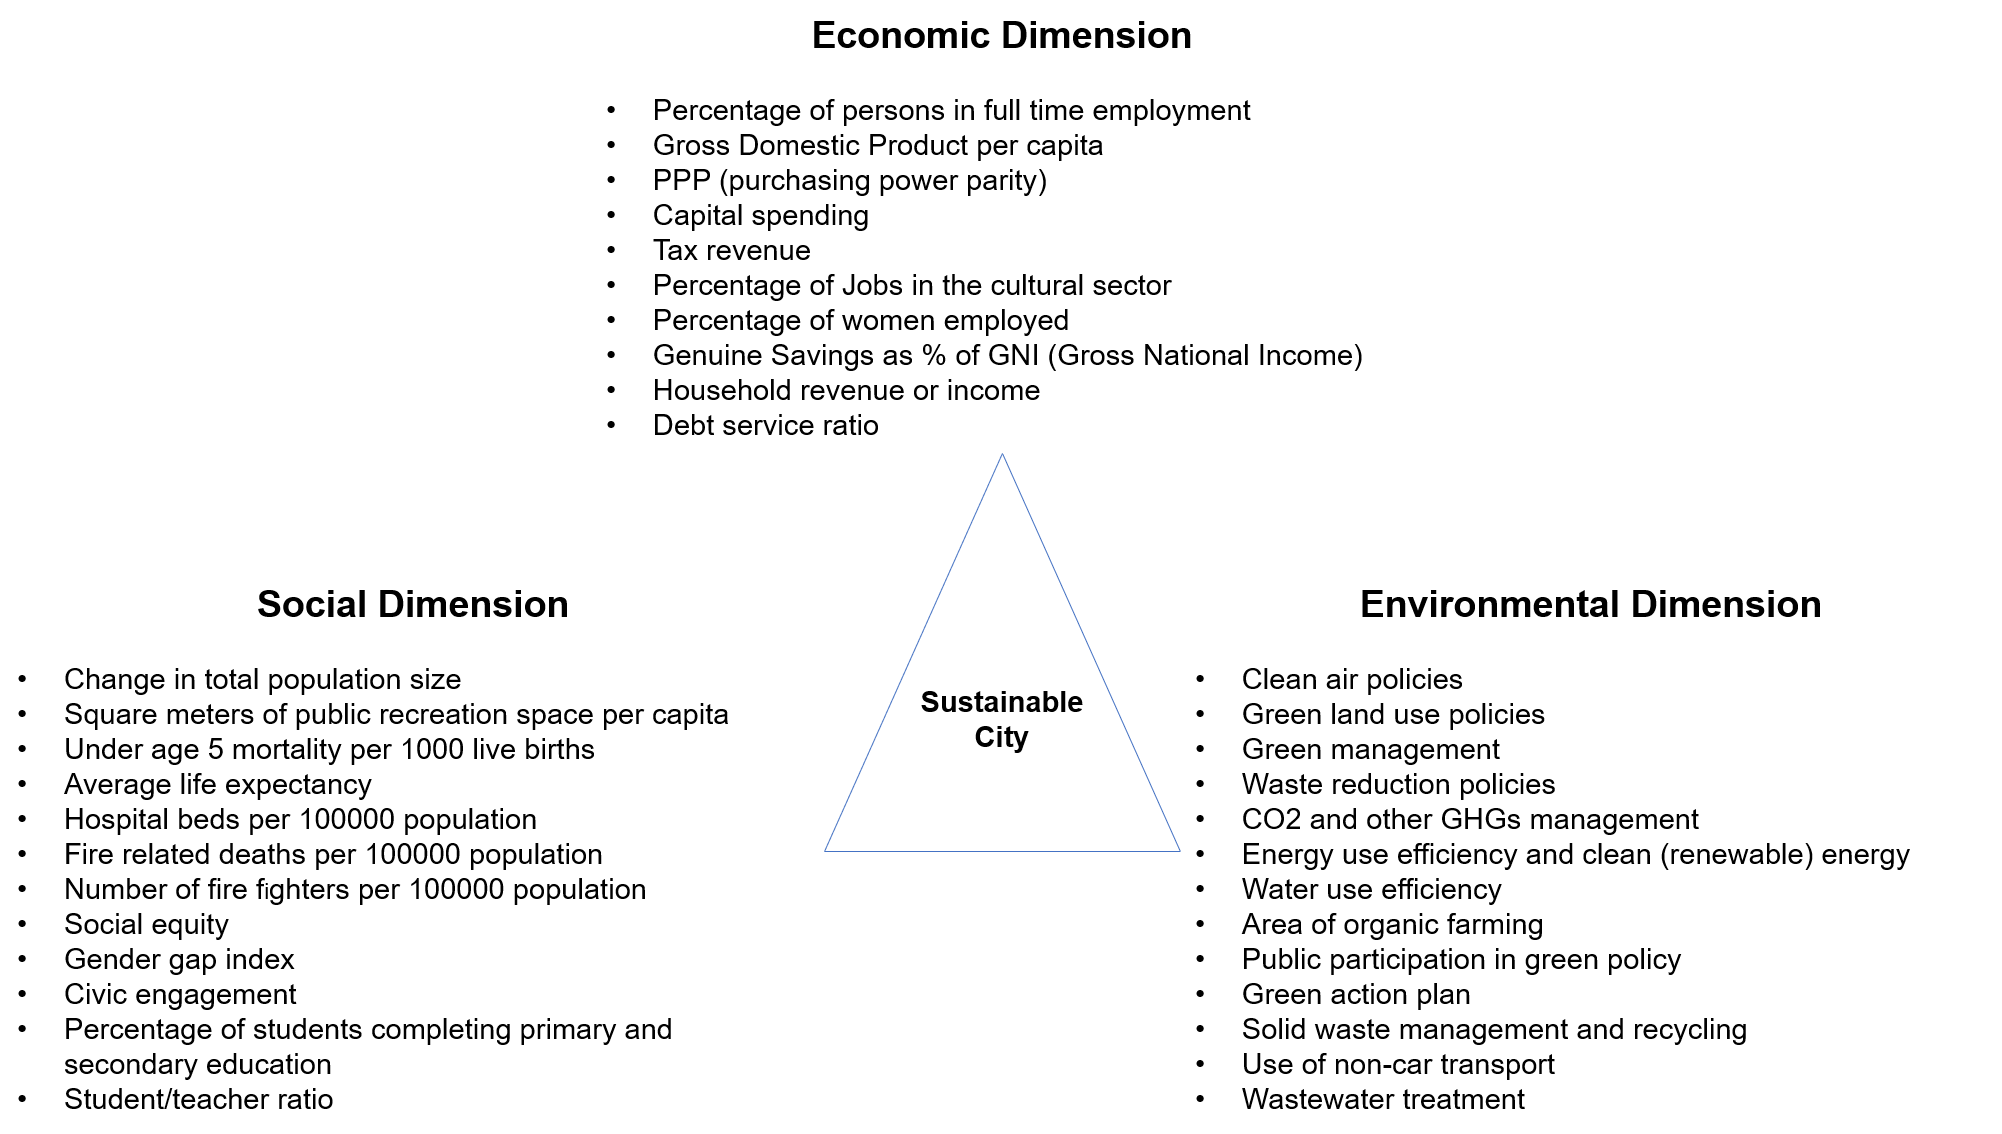
\includegraphics[width=1.00\textwidth]{./Figures/sustainableCityFramework.png}
\decoRule
\caption[Sustainable City Framework]{Sustainable City Framework.}
\label{fig:sustainableCityFramework}
\end{figure}

The report is addressed from several geographical locations with different climatic, economic, social and environmental features. The report intents to state the importance of urban agriculture in the sustainable city. For instance, in the global north, the importance of urban agriculture is more environmental in nature than socio-economic. However, the social and economic functions of urban agriculture are in need within the cities in the global south. Despite the differences, the sustainable city framework in the present report ties together economic, social and ecological indicators and can be applied in every city. The selection of the crops to cultivate to achieve the sustainability goals would be based on the local climatic conditions. On the other hand, the indicators listed in the the sustainable city framework, will be used to identify the impact of Garden Gem in the sustainable city.

\section{Garden Gem Development}

The methodology to follow in order to get the best contribution to urban agriculture is first to develop some surveys that can help having a better and more realistic view of the current situation of the way agriculture is done in cities. 

Once the data has been gathered, the next step is the development of a mobile application that considers all the issues and situations regarding growing plants. The application must be provided by this information so it can give more accurate information related with growing plants.

The next step is for the user to enter the information about the plants that wants to grow. The application must be able to provide the user with a detailed description of the necessary growing conditions in order to make plants grow better despite all conditions that may affect their growing, depending on the issues found for the given plant.

Finally, the application must be tested by real users in order to get the necessary feedback to verify the correct operation of the application. Thus, the development of the application could be validated and considered for furthermore applications.

%\begin{figure}[th]
%\centering
%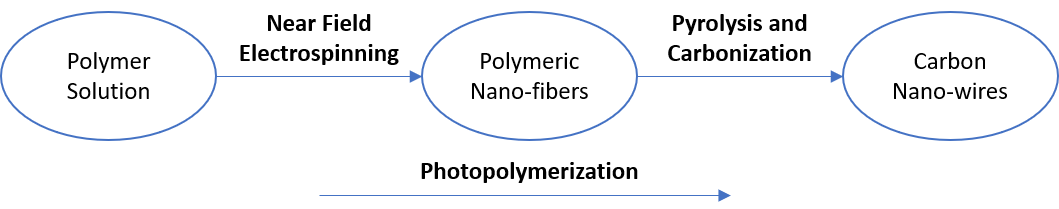
\includegraphics[width=0.95\textwidth]{./Figures/FabricationProcess.png}
%\decoRule
%\caption[Carbon Nano-wires Fabrication Process]{Fabrication process of carbon nano-wires to achieve through the proposed dissertation.}
%\label{fig:fabricationFlowChart}
%\end{figure}

%\begin{equation}
%\left(\tau _t^e-\frac{\tau _n^e \text{dr}}{\text{dz}}\right) 2 \pi  r+\frac{d \left(\pi  r^2
%   \left(\tau _{\text{zz}}-p\right)\right)}{\text{dz}}+\frac{\gamma  \text{dr} 2 \pi  r}{r
%   \text{dz}}+\rho  g \pi  r^2=\frac{d \left(\rho  \pi  r^2 v^2\right)}{\text{dz}}
%\label{eq:linearMomentum}
%\end{equation}